\documentclass{standalone}
\usepackage{tikz}
\usepackage{tikzpeople}

\newcommand{\Enc}{\ensuremath{\mathsf{Enc}}}
\newcommand{\Dec}{\ensuremath{\mathsf{Dec}}}

\begin{document}
			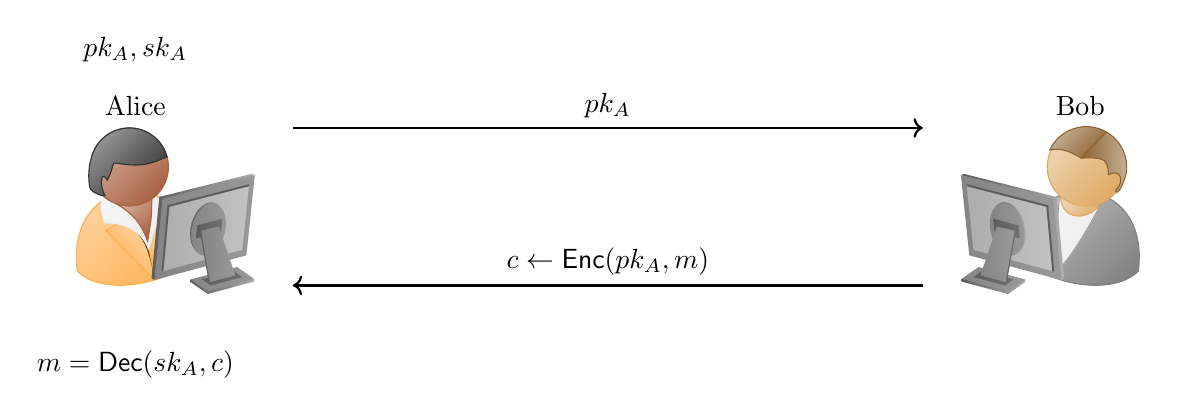
\begin{tikzpicture}
				\node[alice, monitor, label=Alice, minimum size=1.5cm] (Alice) at (0,0) {};
				%			\node[devil, evil, mirrored, label=Attacker, minimum size=1.5cm] (Attacker) at (6,0) {};
				\node[bob, mirrored, monitor, label=Bob, minimum size=1.5cm] (Bob) at (12,0) {};
				\node[] (pkGen) at (0,2) {${pk_A},sk_A$};
				\draw[->, thick] (2,1)  -- (10,1) node[midway, above] {$pk_A$};
				\draw[<-, thick] (2,-1)  -- (10,-1) node[midway, above] {$c \gets \Enc(pk_A,m)$};
				\node[] (dec) at (0,-2) {{$m=\Dec(sk_A,c)$}};
				
			\end{tikzpicture}
\end{document}
